\documentclass[border=3mm,tikz,preview]{standalone}
\usepackage[utf8]{inputenc}
\usepackage{amsmath,amssymb,amsfonts}
\usepackage{graphicx}
\usepackage{tikz}
\usetikzlibrary{shapes.geometric, arrows.meta, positioning, shadows, calc, fit, backgrounds}
\usepackage{xcolor}
\begin{document}

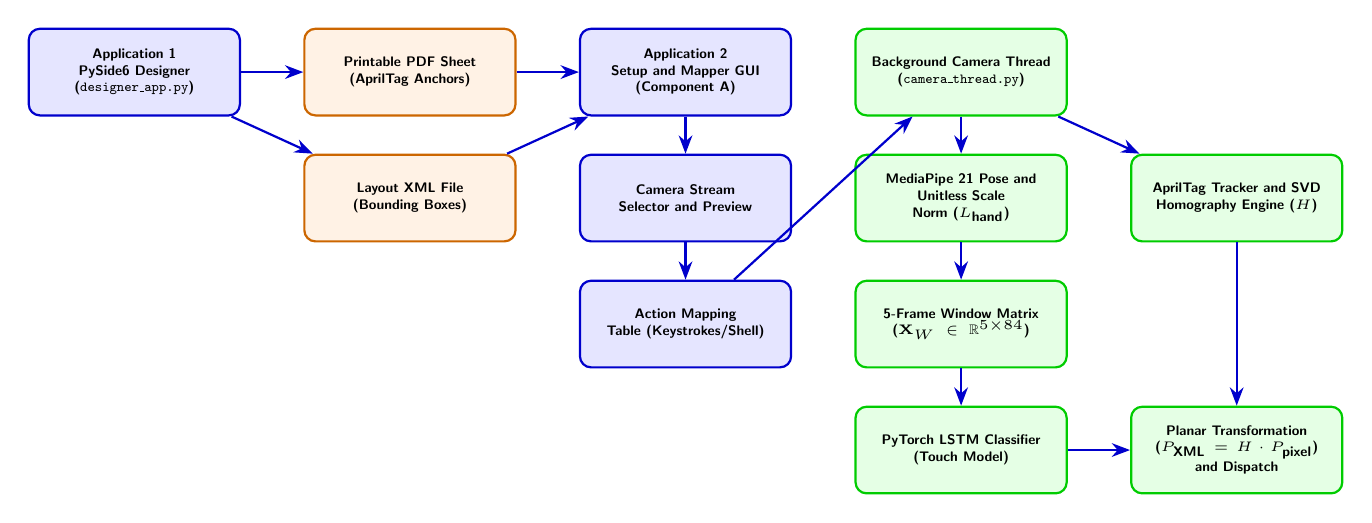
\begin{tikzpicture}[
    node distance = 0.8cm and 0.5cm,
    block/.style = {rectangle, draw=blue!80!black, fill=blue!10!white, thick, rounded corners=4pt, align=center, font=\sffamily\bfseries\tiny, minimum height=1.1cm, text width=2.4cm, inner sep=4pt},
    artblock/.style = {rectangle, draw=orange!80!black, fill=orange!10!white, thick, rounded corners=4pt, align=center, font=\sffamily\bfseries\tiny, minimum height=1.1cm, text width=2.4cm, inner sep=4pt},
    engineblock/.style = {rectangle, draw=green!80!black, fill=green!10!white, thick, rounded corners=4pt, align=center, font=\sffamily\bfseries\tiny, minimum height=1.1cm, text width=2.4cm, inner sep=4pt},
    arrow/.style = {draw=blue!80!black, ->, >=Stealth, thick}
]

% Column 1
\node (b1) [block] at (0, 0) {Application 1\\PySide6 Designer\\(\texttt{designer\_app.py})};

% Column 2
\node (b2) [artblock] at (3.5, 0) {Printable PDF Sheet\\(AprilTag Anchors)};
\node (b3) [artblock] at (3.5, -1.6) {Layout XML File\\(Bounding Boxes)};

% Column 3
\node (b4) [block] at (7.0, 0) {Application 2\\Setup and Mapper GUI\\(Component A)};
\node (b5) [block] at (7.0, -1.6) {Camera Stream\\Selector and Preview};
\node (b6) [block] at (7.0, -3.2) {Action Mapping\\Table (Keystrokes/Shell)};

% Column 4
\node (b7) [engineblock] at (10.5, 0) {Background Camera Thread\\(\texttt{camera\_thread.py})};
\node (b8) [engineblock] at (10.5, -1.6) {MediaPipe 21 Pose and\\Unitless Scale Norm ($L_{\text{hand}}$)};
\node (b9) [engineblock] at (10.5, -3.2) {5-Frame Window Matrix\\($\mathbf{X}_W \in \mathbb{R}^{5 \times 84}$)};
\node (b10) [engineblock] at (10.5, -4.8) {PyTorch LSTM Classifier\\(Touch Model)};

% Column 5
\node (b11) [engineblock] at (14.0, -1.6) {AprilTag Tracker and SVD\\Homography Engine ($H$)};
\node (b12) [engineblock] at (14.0, -4.8) {Planar Transformation\\($P_{\text{XML}} = H \cdot P_{\text{pixel}}$) and Dispatch};

% Arrows
\draw [arrow] (b1) -- (b2);
\draw [arrow] (b1) -- (b3);
\draw [arrow] (b2) -- (b4);
\draw [arrow] (b3) -- (b4);
\draw [arrow] (b4) -- (b5);
\draw [arrow] (b5) -- (b6);
\draw [arrow] (b6) -- (b7);

\draw [arrow] (b7) -- (b8);
\draw [arrow] (b8) -- (b9);
\draw [arrow] (b9) -- (b10);
\draw [arrow] (b10) -- (b12);

\draw [arrow] (b7) -- (b11);
\draw [arrow] (b11) -- (b12);

\end{tikzpicture}

\end{document}
